\scanpage{188}
\mspage{393}

2) \uline{Détermination par} $\alpha_0,\beta_0,f$.

Il y a correspondance biunivoque entre les couples $(g,h)$ satisfaisant (25), et les couples
\[
\tag{31}
(\alpha_0,\beta_0)\qquad
\bigl(\alpha_0\in\Pi_{0,3}^{\wedge\sim}=\Pi_{0,3}^{\wedge}\cdot\{1,\tau_\infty\},\quad
\beta_0\in\Pi_{0,3}^{\wedge}\bigr)
\]
\deleted{\unsure{satisf}} via les relations
\[
\tag{32}
\left\{\begin{aligned}
g&=\alpha_0\rho(\alpha_0)^{-1}=[\alpha_0,\rho]\\
h&=\beta_0\sigma_\infty(\beta_0)^{-1}=[\beta_0,\sigma_\infty]
\end{aligned}\right.
\]
Ainsi, les $u\in\unsure{\mathcal{M}_{0,3}^{!\sim}|\mathcal{N}_{0,3}^{!\sim}}$ correspondent aux systèmes
\[
\tag{33}
(\alpha_0,\beta_0,f)\qquad
\alpha_0\in\Pi_{0,3}^{\sim\wedge},\quad\beta_0,f\in\Pi_{0,3}^{\wedge},\quad
f\ \text{\unsure{déterminé} mod }f\mapsto\ell_0^n f\ (n\in\widehat{\mathbb Z})
\]
satisfaisant la condition \inserted{des lacets} (29), considérée comme condition en $\alpha_0,\beta_0,f$, \deleted{\unsure{en}} y substituant \inserted{à} $g,h$ les valeurs données par (32). La relation s'écrit
\[
\sigma_\infty(\beta_0)\beta_0^{-1}\alpha_0\rho(\alpha_0)^{-1}
=\sigma_\infty(f^{-1})\ell_1^\nu\rho(f)
\]
ou encore
\[
\sigma_\infty(f\beta_0)
\underbrace{\beta_0^{-1}\alpha_0}_{(f\beta_0)^{-1}(f\alpha_0)}
\rho(\inserted{f}\alpha_0\deleted{\unsure{f}})^{-1}
=\ell_1^\nu.
\]
ou encore
\[
\tag{34}
\boxed{(f\alpha_0)\rho(f\alpha_0)^{-1}
=\bigl((f\beta_0)\sigma_\infty(f\beta_0)^{-1}\bigr)\ell_1^\nu}
\]
(relation des lacets en $\alpha_0,\beta_0,f$). Comme pour (29), $\nu\in\widehat{\mathbb Z}$ est uniquement déterminé en termes \unsure{de|des} $\alpha_0,\beta_0$, par la possibilité de trouver $f$ satisfaisant à la relation (34).

L'avantage de l'introduction de $\alpha_0,\beta_0$ au lieu

\scanpage{189}

de $g,h$ est de rendre inutiles (car \unsure{automatiques}) les relations (25), -- il reste la seule relation (34) à vérifier. Les relations (23) décrivant $u$ deviennent ici :
\[
\tag{35}
u(\sigma_\infty)=\operatorname{int}(\beta_0)(\sigma_\infty),\qquad
u(\rho)=\operatorname{int}(\alpha_0)(\rho)
\]

3) \uline{Détermination par} $(\alpha,\beta,f)$.

La forme particulière de (34), où le triple $(\alpha_0\ \beta_0\ f)$ n'intervient que par l'intermédiaire du couple correspondant $(f\alpha_0,f\beta_0)$, conduit à poser
\[
\tag{35}
\alpha=f\alpha_0\deleted{\unsure{=}},\qquad\beta=f\beta_0,
\]
on trouve que les $u\in\mathcal{M}_{0,3}^{!\sim}$ sont déterminés par les triples
\[
\tag{36}
(\alpha,\beta,f)\qquad
\begin{gathered}
\alpha\in\Pi_{0,3}^{\sim\wedge},\quad\beta,f\in\Pi_{0,3}^{\wedge},\quad
\alpha,\beta,f\ \text{modulo}\\
\alpha\mapsto\ell_0^n\alpha,\quad\beta\mapsto\ell_0^n\beta,\quad
f\mapsto\ell_0^n f\ (n\in\widehat{\mathbb Z})\\
\text{(un \uline{même} }n\text{ pour }\alpha,\beta,f\text{)}
\end{gathered}
\]
\margin{Un désavantage est l'indétermination du couple $(\alpha,\beta)$, par $(\alpha,\beta)\longrightarrow(\ell_0^n\alpha,\ell_0^n\beta)$ $(n\in\widehat{\mathbb Z})$, mais c'est un inconvénient mineur, qui \unsure{va être levé} plus bas.}
satisfaisant à la condition
\[
\tag{37}
\boxed{\bigl(\alpha\rho(\alpha)^{-1}\bigr)
=\bigl(\beta\sigma_\infty(\beta)^{-1}\bigr)\cdot\ell_1^\nu}
\]
(\uline{relation des lacets en} $\alpha,\beta$). L'avantage de cette relation est que $f$ n'y figure plus.

On retrouve $\alpha_0,\beta_0,g,h$ en fonction de $\alpha,\beta,f$ par les formules
\[
\tag{38}
\alpha_0=f^{-1}\alpha,\qquad\beta_0=f^{-1}\beta
\]
\[
\tag{39}
g=\alpha_0\rho(\alpha_0)^{-1}
=f^{-1}\bigl(\underbrace{\alpha\rho(\alpha)^{-1}}_{\deleted{\illegible{1}}}\bigr)\rho(f)
=f^{-1}\xi\rho(f)
\]
\[
\tag{40}
h=\beta_0\sigma_\infty(\beta_0)^{-1}
=f^{-1}\bigl(\beta\sigma_\infty(\beta)^{-1}\bigr)
=f^{-1}\eta\sigma_\infty(f),
\]
où on a posé
\[
\tag{41}
\xi=\alpha\rho(\alpha)^{-1},\qquad
\eta=\beta\sigma_\infty(\beta)^{-1}
\qquad(\xi,\eta\in\Pi_{0,3}^{\wedge})
\]

\scanpage{190}
\mspage{394}

Les formules (23) -- (35) déterminant $u$ en termes des données \unsure{calculatoires}, deviennent ici
\[
\tag{42}
u(\sigma_\infty)=\operatorname{int}(f^{-1}\beta)(\sigma_\infty)
\qquad u(\rho)=\operatorname{int}(f^{-1}\alpha)(\rho)
\]
\inserted{i.e.
\[
\tag{42bis}
\text{\deleted{\unsure{i.e.}}}\ u=\operatorname{int}(f^{-1})u_{\alpha,\beta},
\]
où $u_{\alpha,\beta}$ ne dépend que de $\alpha,\beta$ :
\[
\tag{42ter}
\boxed{u_{\alpha,\beta}(\sigma_\infty)=\operatorname{int}(\beta)(\sigma_\infty)=\unsure{\eta\sigma_\infty}}
\quad
\boxed{u_{\alpha,\beta}(\rho)=\operatorname{int}(\alpha)(\rho)=\xi\rho}
\]}
La formule (37) \unsure{peut s'interpréter comme une} relation en $\xi,\eta$
\[
\tag{43}
\xi=\eta\ell_1^\nu.
\]

4) \uline{Détermination par} $(\xi,\eta,f)$.

La donnée du couple $(\alpha,\beta)\in\Pi_{0,3}^{\overset{\inserted{\wedge}}{\sim}\wedge}\times\Pi_{0,3}^{\wedge}$, équivaut à celle du couple $(\xi,\eta)$ qui s'en déduit par (41), \unsure{assujetti} aux \deleted{formules}\inserted{équations}
\[
\tag{44}
\boxed{\left\{\begin{aligned}
\xi\rho(\xi)\rho^2(\xi)&=1\\
\eta\sigma_\infty(\eta)&=1
\end{aligned}\right.}
\]
Ainsi, la donnée de $u\in\mathcal{M}_{0,3}^{!\sim}$ équivaut à celle d'un triplet
\[
\tag{45}
(\xi,\eta,f)\qquad
\begin{gathered}
\xi,\eta,f\in\Pi_{0,3}^{\wedge}\quad\text{modulo}\\
\xi\mapsto\ell_0^n\xi\unsure{\ell_1^n|\ell_1^{-n}},\quad
\eta\mapsto\ell_0^n\eta\unsure{\ell_1^n|\ell_1^{-n}},\quad
f\mapsto\ell_0^n f
\end{gathered}
\]
satisfaisant les relations (44), et la relation
\[
\tag*{(46)=(43)}
\boxed{\xi=\eta\ell_1^\nu},
\]
qui joue le rôle de ``\uline{relation des lacets en} $\xi,\eta$''. L'avantage de cette présentation est

\scanpage{191}

la simplicité maximale des équations (44),(46) -- et le fait que $f$ n'y intervienne pas: \deleted{\unsure{ce sont}} les deux premières équations sont des équations en $\xi$ seul et en $\eta$ seul, et la troisième relie $\xi$ et $\eta$ de façon particulièrement simple -- en fait si $\mu=1$, i.e. $\nu=0$, c'est la relation $\xi=\eta$ !

L'inconvénient est qu'il y a trois équations au lieu d'une, et qu'on n'a pas d'expression explicite de $u(\sigma_\infty)$ et de $u(\rho)$ en termes de $\xi,\eta,f$ : il faut d'abord, pour cela, résoudre les équations
\margin{mais si, on a une belle \unsure{expression} explicite (42ter) :
\[
u(\sigma_\infty)=\operatorname{int}(f^{-1})(\eta\sigma_\infty)
\]
\[
u(\rho)=\operatorname{int}(f^{-1})(\xi\rho)
\]
!!}
\[
\tag{47}
\left\{\begin{aligned}
\alpha\rho(\alpha)^{-1}&=\xi\qquad(\alpha\in\Pi_{0,3}^{\sim\wedge})\\
\beta\sigma_\infty(\beta)^{-1}&=\eta\qquad(\beta\in\Pi_{0,3}^{\wedge})
\end{aligned}\right.
\]
en $\alpha,\beta$, pour pouvoir ensuite appliquer (42).

Un autre \inserted{[!]} inconvénient, d'importance, c'est que lorsqu'on travaille avec les images des éléments envisagés dans $\mathrm{Gl}(2,\widehat{\mathbb Z})^{\unsure{\pm\prime|\pm1}}$, la connaissance dans ce groupe de $\xi,\eta$ \inserted{(même dans $\mathrm{Sl}(2,\widehat{\mathbb Z})$ lui-$\overline{\mathrm m}$)} est \deleted{\unsure{trop}} une donnée assez faible, qui ne permet nullement de retrouver $\alpha,\beta$ comme éléments de $\mathrm{Gl}(2,\widehat{\mathbb Z})^{\unsure{\pm\prime|\pm1}}$, cf plus bas.

\scanpage{192}
\mspage{395}

5) \uline{Composition \unsure{aux|avec} autom.} \uline{intérieurs}. \uline{Relations des cocycles} \uline{pour un composé} $u''=u'u$.

Soit $\gamma\in\Pi_{0,3}^{\wedge}$, et considérons le composé
\[
\tag{48}
u'=\operatorname{int}(\gamma)\circ u
\]
il correspond à des invariants
\[
f',g',\unsure{h'|\beta'},\alpha_0',\beta_0',\alpha',\beta',\xi',\eta'
\]
donnés par
\[
\tag{49}
\left\{\begin{aligned}
f'&=f\gamma^{-1},\quad\deleted{\unsure{g'=\gamma g},\ h'=\gamma h}\\
g'&=\gamma g\rho(\gamma)^{-1},\quad h'=\gamma h\sigma_\infty(\gamma)^{-1}\\
\alpha_0'&=\gamma\alpha_0,\quad\beta_0'=\gamma\beta_0\\
\alpha'&=\alpha,\quad\beta'=\beta\\
\xi'&=\xi,\quad\eta'=\eta
\end{aligned}\right.
\]
Ainsi $\alpha$ et $\beta$ ne changent pas quand on remplace $\unsure{u|f}$ par $\operatorname{int}(\gamma)u$, ils ne dépendent que de l'autom ext. à lacets défini par $u$, i.e. de l'image de $u$ dans $\mathcal{N}_{0,3}^{!\sim}$. C'est là un avantage substantiel de l'utilisation de $(\alpha,\beta,f)$ ou de $(\xi,\eta,f)$, de préférence à $(\alpha_0,\beta_0,f)$ ou de $(g,h,f)$.

Soient maintenant
\[
\tag{50}
u,u'\in\mathcal{M}_{0,3}^{!\sim},\quad\text{soit }u''=u'u
\]
soient
\[
\tag{51}
\left\{\begin{aligned}
&f,g,h,\alpha_0,\beta_0,\alpha,\beta,\xi,\eta\\
&f',g',h',\alpha_0',\beta_0',\alpha',\beta',\xi',\eta'\qquad\unsure{\text{et}}\\
&f'',g'',h'',\alpha_0'',\beta_0'',\alpha'',\beta'',\xi'',\eta''
\end{aligned}\right.
\]

\scanpage{193}

les invariants relatifs à $u,u',u''$ respectivement, -- on \unsure{veut} exprimer (dans la mesure du possible) ceux de $u''$ en fonction de ceux de $u,u'$, et on trouve
\[
\begin{aligned}
&\left\{\begin{array}{lll}
g''=u'(g)g' & \alpha_0''=u'(\alpha_0)\alpha_0'\, {*} & \alpha''=\unsure{(f'u')}(\alpha).\alpha'\, {*}\\
h''=u'(h)h' & \beta_0''=u'(\beta_0)\beta_0' & \beta''=(f'u')(\beta).\beta'
\end{array}\right.\\
&\text{mais } f''=f'u'(f)\deleted{\unsure{\xi}}.
\end{aligned}
\tag{52}
\]
\margin{${*}$ $u'(\alpha_0)$ et $(f'u')(\alpha)$ n'ont de sens a priori que si $\alpha_0,\alpha\in\widehat{\Pi}_{0,3}$ i.e. $\mu\equiv1\ (3)$, sinon (p.ex.) on peut encore définir $u'(\alpha_0)=u'\alpha_0u'^{-1}$, mais il ne sera plus \deleted{\unsure{dans}} \illegible{2} dans $\widehat{\Pi}_{0,3}$, et la formule $\alpha_0''=u'(\alpha_0)\alpha_0'$ aura un sens, mais sera \uline{fausse} !}

On voit donc que si on considère \unsure{(pour} $u$ variable dans $\mathcal M_{0,3}^{!\sim})$ $f,g,h,\alpha_0,\beta_0,\alpha,\beta$ comme des fonctions
\[
\mathcal M_{0,3}^{!\sim}\longrightarrow\widehat{\Pi}_{0,3},\ \text{ou }\widetilde{\Pi}_{0,3}^{\wedge}
\]
alors $f,g^{-1},h^{-1},\alpha_0^{-1},\beta_0^{-1}$ satisfont la relation des \uline{cocycles}, et $\alpha^{-1},\beta^{-1}$ aussi quand on se limite au\deleted{\illegible{1}} sous-groupe pour lequel $f=1$, i.e. les autom. $u\in\mathcal M_{0,3}^{!\sim}$ qui \uline{normalisent} \deleted{\unsure{le}} $L_0=\{\ell_0^n\mid n\in\widehat{\mathbb Z}\}$. A' vrai dire, cet énoncé \inserted{\deleted{\illegible{1}} pour $f$, $\alpha$, $\beta$} est un peu boiteux, à cause des indéterminations pour $f$, impliquant une indétermination correspondante pour $\alpha,\beta$, $f\mapsto\ell_0^n f$, $\alpha\mapsto\ell_0^n\alpha$, $\beta\mapsto\ell_0^n\beta$. Pour construire des cocycles canoniques correspondant à $f,\alpha^{-1},\beta^{-1}$, il faud\inserted{rait} introduire un groupe extension de $\mathcal M_{0,3}^{!\sim}$ par $\widehat{\mathbb Z}$, sur le modèle des groupes de Teichmüller spéciaux, sur lequel $f,\alpha,\beta$ soient définis sans ambiguité. Ça ne s'impose pas ici de détailler\ldots

\scanpage{194}
\mspage{396}

\uline{$\overline{\mathrm{III}}$}\quad \uline{Calculs dans} $\mathrm{Gl}(2,\widehat{\mathbb Z})'$ \uline{et dans} $\mathrm{Gl}(2,\widehat{\mathbb Z})$.

Pour $u\in\mathcal M_{0,3}^{!\sim}$ donné, d'où les quantités
\[
f,g,h,\alpha_0,\beta_0,\alpha,\beta,\xi,\eta:
\tag{53}
\]
(toutes dans $\widehat{\Pi}_{0,3}$, sauf $\alpha_0,\alpha$ qui ne sont que dans $\widetilde{\Pi}_{0,3}^{\wedge}\simeq\widehat{\Pi}_{0,3}.\{1,\tau_\infty\}$) on désigne par les \unsure{mêmes lettres} \unsure{les|leurs} images dans \deleted{$\mathrm{Gl}(2,\widehat{\mathbb Z})$}
\[
\mathrm{Gl}(2,\widehat{\mathbb Z})'\stackrel{\mathrm{dfn}}{=}\mathrm{Gl}(2,\widehat{\mathbb Z})/\mathord{\pm}1,
\]
elles sont en fait dans
\[
\mathrm{Sl}(2,\widehat{\mathbb Z})'=\mathrm{Sl}(2,\widehat{\mathbb Z})/\mathord{\pm}1,
\]
\unsure{sauf} $\alpha_0,\alpha$ qui sont seulement dans $\mathrm{Gl}(2,\widehat{\mathbb Z})^{\unsure{\pm'|\pm1}}$
\[
\det\alpha_0=\det\alpha=\varepsilon_3\in\{\pm1\}
\tag{54}
\]
où $\varepsilon_3$ est défini par
\[
\varepsilon_3\equiv\mu\quad(3),
\tag{55}
\]
\illegible{1} par ailleurs.
\[
\begin{gathered}
f,g,h,\beta_0,\beta,\xi,\eta\in\mathrm{Sl}(2,\widehat{\mathbb Z})'\quad\text{i.e.}\\
\det f=\det g=\det h=\det\beta_0=\det\beta=\det\xi=\det\eta=1
\end{gathered}
\tag{56}
\]
\margin{NB $f$ est déterminé mod transformation en $\ell_0^n f$, et par là $\alpha,\beta$ sont affectés de la $\overline{\mathrm m}$ indétermination -- de façon plus précise on a une indétermination $(\alpha,\beta,f)\mapsto(\ell_0^n\alpha,\ell_0^n\beta,\ell_0^n f)$, (en plus de celle des signes). Dans ce qui suit, on \unsure{supposera} donc \deleted{\illegible{1}} \inserted{$f,\alpha,\beta$} \uline{choisis} dans $\widehat{\Pi}_{0,3}$, et que les images dans $\mathrm{Gl}(2,\widehat{\mathbb Z})'$ ont été \unsure{relevées} dans $\mathrm{Gl}(2,\widehat{\mathbb Z})$\ldots}
\margin{cf p.\unsure{398|348} \unsure{ou mieux|en mieux} formulaire plus bas}

(\uline{NB} \unsure{On} \deleted{\unsure{fonction}} $\det(-1)=1$, donc $\det$ se factorise
\[
\mathrm{Gl}(2,\widehat{\mathbb Z})'\xrightarrow{\det}\widehat{\mathbb Z}^{\times},
\]
pour donner une suite exacte
\[
1\longrightarrow\mathrm{Sl}(2,\widehat{\mathbb Z})'\unsure{\longrightarrow}\mathrm{Gl}(2,\widehat{\mathbb Z})'\longrightarrow\widehat{\mathbb Z}^{\times}\unsure{\longrightarrow}1
\tag{57}
\]
).

On choisira des représentants
\[
f,\unsure{\alpha|\alpha_0},\unsure{\beta_0|\beta}\in\mathrm{Gl}(2,\widehat{\mathbb Z})
\tag{58}
\]
ce qui équivaut au choix de \uline{trois} \uline{signes},

\scanpage{195}

et en fonction de ces choix on définit les autres quantités par
\[
\deleted{\left\{\begin{array}{ll}
g=\alpha_0\rho(\alpha_0)^{-1},&h=\beta_0\sigma_\infty(\beta_0)^{-1},\quad\text{et}\\
\alpha_0=f^{-1}\unsure{\alpha_0|\alpha},&\beta_0=f^{-1}\unsure{\beta_0|\beta},\\
\xi=\alpha\rho(\alpha)^{-1},&\eta=\beta\rho(\beta)^{-1}
\end{array}\right.}
\]
\[
\left\{\begin{array}{ll}
\xi=\alpha\rho(\alpha)^{-1},&\eta=\beta\deleted{\unsure{\rho}}\inserted{\sigma_\infty}(\beta)^{-1}\\[4pt]
\alpha_0=f^{-1}\alpha,&\beta_0=f^{-1}\beta\\[8pt]
g=\alpha_0\rho(\alpha_0)^{-1}=f^{-1}\xi\rho(f),&h=\beta_0\rho(\beta_0)^{-1}=f^{-1}\eta\rho(f).
\end{array}\right.
\tag{59}
\]

On \unsure{notera} que $\xi$ et $\eta$, \deleted{\unsure{ou}} $g,h$ sont indépendants du choix des signes qui ont été faits. La relation essentielle qui relie $(f,\unsure{\alpha_0|\alpha},\unsure{\beta_0|\beta})$, ou plutôt $\alpha,\beta$ (en plus des relations (59), qui jouent le rôle de relations de définition) est la ``relation des lacets'', sous forme matricielle, qui prend la forme (correspondant à (46) ou à (43))
\[
\boxed{\xi=\varepsilon\eta\ell_1^\nu}\qquad\varepsilon\in\{\pm1\}
\tag{60}
\]
où $\varepsilon\deleted{\unsure{\varepsilon_2}}$ est un signe qui ne dépend plus d'aucun choix -- \unsure{on a vu|on a en} \deleted{\illegible{1}} (cf aussi formulaire plus bas)
\[
\varepsilon=\varepsilon_2\quad
\text{défini en termes }\inserted{\unsure{\text{i.e.}}}\text{ de }\mu\text{ par }\quad
\mu\equiv\varepsilon_2\quad(4),
\tag{61}
\]

\scanpage{196}
\mspage{397}

et où $\ell_1$ est défini matriciellement par
\[
\deleted{\unsure{(62)}}\qquad
\ell_1=\begin{pmatrix}1&0\\2&1\end{pmatrix}
\]
d'où
\[
\ell_1^\nu=\begin{pmatrix}1&0\\2\nu&1\end{pmatrix}
=\begin{pmatrix}1&0\\\mu-1&1\end{pmatrix}.
\tag{62}
\]

\uline{Remarque}

(Relation avec les notations du \S\,44 (p.356 ff, notamment formulaire après p.364). Dans les groupes $\widehat{\Pi}_{0,3}$ et $\widetilde{\Pi}_{0,3}^{\wedge}$, les lettres $f,g,h$ de loc. cit. \unsure{ont|sont} le $\overline{\mathrm m}$ sens qu'ici, mais non les lettres $\alpha,\beta$ etc. Je vais distinguer par des soulignés, dans le cas de \unsure{déviation} \inserted{entre les deux notations}, les lettres avec la \deleted{\unsure{sens}} signification \unsure{utilisée|étudiée} dans loc. cit, on trouve
\[
\uline{\alpha}=\alpha_0,\qquad\uline{\beta}=\beta_0
\tag{i}
\]
à partir de p.357 on suppose pratiquement tjrs $\uline{\beta}=\beta_0=1$, \inserted{(i.e. $u(\sigma_\infty)=\sigma_\infty$)} de sorte que
\[
\boxed{\beta=f\beta_0=f}
\tag{ii}
\]
\deleted{et} et loc. cit (17) donne
\[
\uline{\varphi}=f\sigma_\infty(f)^{-1}=\beta\sigma_\infty(\beta)^{-1}=\eta
\tag{iii}
\]
tandis que (\unsure{loc.} cit (14))
\[
\uline{\xi}=\ell_0^\nu\uline{\varphi}=\ell_0^\nu\eta,
\]
en comparant avec
\[
\xi=\eta\ell_1^\nu\qquad(46)
\]
on trouve
\[
\deleted{\unsure{(iv)}}\quad\uline{\xi}=\ell_0^\nu\xi\ell_1^{-\nu}
=\ell_0^\nu\xi\rho(\ell_0^\nu)^{-1}.
\tag{iv}
\]
i.e. $\uline{\xi}$ est le $\rho$-transformé de $\ell_0^\nu$.
La relation (loc. cit (\unsure{19|29}))
\[
\uline{\xi}=\uline{\alpha}_0\rho(\uline{\alpha}_0)^{-1}
\]
comparée à $\xi=\alpha\rho(\alpha)^{-1}$ et à (iv)\deleted{\illegible{1}}, donne

\scanpage{197}

\[
\deleted{(\illegible{1})}\qquad\uline{\alpha}_0=\ell_0^\nu\alpha.
\tag{v}
\]

Les formules \deleted{\illegible{2}} \inserted{(i) à (v)} permettent de traduire le formulaire de loc. cit. en termes du formulaire que je vais expliciter.

On explicite $\alpha$ et $\beta$ par leurs matrices
\[
\alpha=\begin{pmatrix}a&b\\c&d\end{pmatrix},\qquad
\beta=\begin{pmatrix}r&s\\t&u\end{pmatrix},
\tag{63}
\]
où $a,b,c,d,r,s,t,u\in\widehat{\mathbb Z}$, avec
\[
ad-bc=\deleted{\varepsilon_{\illegible{1}}}\inserted{\delta}=\varepsilon_3,\qquad ru-st=1.
\tag{64}
\]
on aura
\[
\xi=\alpha\rho(\alpha)^{-1}=\begin{pmatrix}A&B\\C&D\end{pmatrix}
\tag{65}
\]
avec (cf. p.342, \unsure{(78)|(18)})
\[
\left\{\begin{array}{ll}
\delta A=(a^2+ab+b^2)-(ac+bd+bc),&\delta B=ac+bd+bc\\[4pt]
\delta C=-(c^2+cd+d^2)+(ac+bd+ad),&\delta D=c^2+cd+d^2
\end{array}\right.,
\tag{66}
\]
\[
\eta=\beta\sigma_\infty(\beta)^{-1}=\begin{pmatrix}R&S\\T&U\end{pmatrix},\quad\text{avec}
\tag{67}
\]
\[
R=r^2+s^2,\quad S=T=rt+su,\quad U=t^2+u^2.
\tag{68}
\]
La relation des lacets (60) prend la forme
\[
\begin{aligned}
\begin{pmatrix}A&B\\C&D\end{pmatrix}
&=\varepsilon\begin{pmatrix}R&S\\T&\deleted{\unsure{T}}\inserted{U}\end{pmatrix}
\begin{pmatrix}1&0\\2\nu&1\end{pmatrix}\\[4pt]
&=\varepsilon\begin{pmatrix}R+2\nu S&S\\T+2\nu U&U\end{pmatrix},
\end{aligned}
\tag*{\boxed{(69)}}
\]

\scanpage{198}
\mspage{398}

Notons les relations (\unsure{conséquences} de (66), (67)) :
\[
(70)\qquad AD-BC=1\qquad RU-ST=1
\]
\[
(71)\qquad C+D-B=1\qquad T\unsure{=|-}S=1\quad\text{i.e. }T=S,
\]
Cette relation des \deleted{\unsure{cocycles}}\inserted{lacets} (69) \deleted{prend} est équivalente au système de relations
\[
(72)\qquad
\boxed{\begin{gathered}
D=\varepsilon U\\
\mu D=1\\
B=\varepsilon S
\end{gathered}}
\qquad(\text{où }\mu=2\nu+1),
\]
i.e. au système d'équations
\[
(73)\qquad
\left\{\begin{aligned}
c^2+cd+d^2&=\varepsilon(t^2+u^2)=\delta/\mu\\
ac+bd+bc&=\varepsilon(rt+su)\\
&\deleted{\mu(c^2+cd+d^2)=\delta}
\end{aligned}\right.
\]
C'est \unsure{des|de} \deleted{\unsure{la comparaison de la première}}\inserted{deux premières relations} (73) que l'on tire aussitôt
\[
(74)\qquad\delta\equiv\mu\ (3),\qquad\varepsilon\equiv\mu\ (4)
\]
qui caractérisent les signes $\delta,\varepsilon$ comme
\[
(75)\qquad\delta=\varepsilon_3(\mu)=\varepsilon_3,\qquad
\varepsilon=\varepsilon_2(\mu)=\varepsilon_2,
\]
cf \unsure{Th.} p. 365.

La formule (83) de la page 370 prend ici la forme très simple (valable sans conditions autres que celles \unsure{précisées} jusqu'ici sur $\alpha,\beta,f$ --- $f$ n'intervenant d'ailleurs pas \deleted{\unsure{dans}} pour le moment dans le formulaire) :

\scanpage{199}

\[
(76)\qquad
\underset{\substack{\Vert\\\varepsilon_3\in\{\pm1\}}}{(\delta)}
\alpha(c\rho+d)=\beta(t\sigma_\infty+u)\tau_\infty^{\alpha_2}
\qquad(\alpha=\alpha_2)
\]
où $\alpha_2=\alpha$ est défini par la condition
\[
(-1)^{\alpha_2}=\varepsilon\quad(=\varepsilon_2).
\]
Explicitant (76) par le calcul matriciel, on a
\[
\delta\alpha(c\rho+d)
=\delta\begin{pmatrix}a&b\\c&d\end{pmatrix}
\begin{pmatrix}d&c\\-c&c+d\end{pmatrix}
=\deleted{\unsure{\delta}}
\begin{pmatrix}1&B\\0&D\end{pmatrix}
\]
\[
\beta(t\sigma_\infty+u)\tau_\infty^\alpha
=\begin{pmatrix}\unsure{r}&\unsure{s|-s}\\\unsure{t|-t}&u\end{pmatrix}
\begin{pmatrix}u&\unsure{\varepsilon_2t|\varepsilon t}\\-t&\varepsilon u\end{pmatrix}
=\begin{pmatrix}1&\varepsilon S\\0&\varepsilon U\end{pmatrix}
\]
de sorte que (76) se réduit aux équations
\[
D=\varepsilon U,\quad B=\varepsilon S,
\]
donc \uline{la relation des lacets} $\xi=\varepsilon\eta \ell_1^\nu$ (\unsure{60|68}, 69) \uline{est équivalente} à \uline{la conjonction de} (76) et de la relation
\[
(77)\qquad\mu D=1.
\]
Ceci posé, on posera \inserted{(pour $(\alpha,\beta)$ fixés de façon à satisfaire la formule des lacets)}
\[
\begin{aligned}
(78)\qquad u_{\alpha,\beta}
&\overset{\mathrm{dfn}}{=}(\mu\delta).\alpha(c\rho+d)
=\mu\beta(t\sigma_\infty+u)\tau_\infty^\alpha\\
&=\mu\begin{pmatrix}1&B\\0&D\end{pmatrix}
=\begin{pmatrix}\mu&\mu B\\0&1\end{pmatrix}
\end{aligned}
\]
de façon que $u_{\alpha,\beta}$ ne dépend en fait que de $\alpha$, ou que de $\beta$ et du signe $\alpha_2$ (qui, lui, n'est pas déterminé par $\beta$, mais par $\alpha$ comme la valeur de $\delta(c^2+cd+d^2)\bmod4$\dots); et on posera, pour un triple $(\alpha,\beta,f)$ d'éléments de $\mathrm{Gl}(2,\widehat{\mathbb Z})$, $\det f=1$, $\unsure{\alpha\text{ et }\beta|\det\beta}$ reliés par la formule des lacets

\margin{en fait, $u_{\alpha\beta}$ ne dépend que de $\xi=\alpha\rho(\alpha)^{-1}$, et $\overline{\mathrm m}$ seulement de l'image $\unsure{\overline\xi|\xi}$ de $\xi$ dans $\unsure{\mathrm{Sl}(2,\widehat{\mathbb Z})|\mathrm{Sl}(2,\widehat{\mathbb Z})'}$, \unsure{le signe étant caractérisé} par la condition $\xi\rho(\xi)\rho^2(\xi)=+1$) i.e. ne dépend que de $\unsure{B,D(=1/\mu\dots)}$. Il faudrait le noter $u_\xi$, cf. p. 410.}

\scanpage{200}
\mspage{399}

\[
\begin{aligned}
(79)\qquad u_{\alpha,\beta,f}
&\overset{\mathrm{dfn}}{=}f^{-1}u_{\alpha,\beta}
=(\mu\delta)\overbrace{f^{-1}\alpha}^{\alpha_0}(c\rho+d)=\\
&=\mu\underbrace{f^{-1}\beta}_{\beta_0}(t\sigma_\infty+u)\tau_\infty^{\alpha_2}
\end{aligned}
\]
et on trouve, comme il se doit,
\[
(80)\qquad
\left\{\begin{aligned}
u_{\alpha,\beta,f}(\sigma_\infty)&=\operatorname{int}(\beta_0)(\sigma_\infty)\\
u_{\alpha,\beta,f}(\rho)&=\operatorname{int}(\unsure{\alpha_0|\beta_0})(\rho)
\end{aligned}\right.,
\]
\margin{\figure{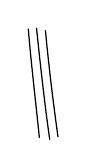
\begin{tikzpicture}[x=1mm,y=1mm,line width=.45pt,line cap=round]
\draw (0,14.0) .. controls (.36,9.6) and (1.02,4.1) .. (1.40,.25);
\draw (1.05,14.1) .. controls (1.53,9.4) and (2.14,4.0) .. (2.72,0);
\draw (2.18,13.8) .. controls (2.62,9.0) and (3.26,4.0) .. (3.77,.32);
\end{tikzpicture}}}
\margin{\uline{NB} \unsure{si|Si} $u,\sigma$ sont des éléments d'un groupe $G$, on pose bien sûr $u(\sigma)=u\sigma u^{-1}$.}
\margin{ceci \uline{implique que}, \deleted{\unsure{par}} $\operatorname{int}(u_{\alpha,\beta,f})$ a même effet, \unsure{sur|en} $\mathrm{Sl}(2,\widehat{\mathbb Z})'$ que l'\unsure{autom} $u$ de $\unsure{\widehat{\mathcal G}_{0,3}^{+}|\widetilde{\mathcal G}_{0,3}^{\to}}$ défini (quand il y en a un), par passage au quotient en $\mathrm{Sl}(2,\widehat{\mathbb Z})'$.}

formules qui se réduisent à des formules où $f$ à nouveau a disparu
\[
(81)\qquad
\left\{\begin{aligned}
u_{\alpha,\beta}(\sigma_\infty)&=\operatorname{int}(\beta)(\sigma_\infty)\\
u_{\alpha,\beta}(\rho)&=\operatorname{int}(\unsure{\alpha|\beta})(\rho)
\end{aligned}\right.,
\]
qui \deleted{à leur tour} résultent \inserted{\uline{trivialement}} des deux expressions \deleted{de} (78) de $u_{\alpha,\beta}$ !

Les formules (80) se complètent de façon naturelle en
\[
(82)\qquad
u_{\alpha,\beta,f}(\varepsilon_0)
=\deleted{\unsure{f\varepsilon_0}}\inserted{\varepsilon}\operatorname{int}(f^{-1})(\varepsilon_0^\mu)
\qquad\deleted{\unsure{(\varepsilon=\varepsilon_2)}}
\]
\[
(\text{où }\varepsilon=\varepsilon_2\in\{\pm1\})
\]
\margin{\figure{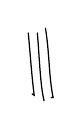
\begin{tikzpicture}[x=1mm,y=1mm,line width=.45pt,line cap=round]
\draw (0,8.6) .. controls (.28,5.5) and (.48,2.7) .. (.75,.7) -- (.48,.86);
\draw (1.15,8.6) .. controls (1.44,5.1) and (1.52,2.0) .. (2.0,0);
\draw (2.18,9.2) .. controls (2.68,6.2) and (2.62,2.9) .. (3.15,.43) -- (2.90,.39);
\end{tikzpicture}}}
qui à son tour se réduit à
\[
(83)\qquad u_{\alpha,\beta}(\varepsilon_0)=\varepsilon.\varepsilon_0^\mu
\]
où $f$ ne figure plus. Comme $\varepsilon_0=\sigma_\infty\rho$, cette formule se réduit à :
\[
u_{\alpha,\beta}(\sigma_\infty)u_{\alpha,\beta}(\rho)=\varepsilon.\varepsilon_0^\mu,
\]
qui compte tenu de (81) se réduit à :
\[
\operatorname{int}(\beta)(\sigma_\infty)\operatorname{int}(\unsure{\alpha|\beta})(\rho)=\varepsilon.\varepsilon_0^\mu
\]
\deleted{\unsure{puis}}
\[
\deleted{\unsure{\alpha\sigma_\infty\alpha^{-1}\beta\rho\beta^{-1}}}
\]

\scanpage{201}

or le premier \unsure{mb} s'écrit
\[
\deleted{\unsure{\beta\sigma_\infty\beta^{-1}\alpha\rho\alpha^{-1}
=(\beta\sigma_\infty\beta^{-1}\sigma_\infty)(\sigma_\infty\rho)(\rho^{-1}\alpha\rho\alpha^{-1})}}
\]
\[
\deleted{\unsure{=(\beta\sigma_\infty(\beta)^{-1})\varepsilon_0(\rho^{-1}(\alpha)\beta^{-1})}}
\]
\[
\begin{aligned}
\beta\sigma_\infty\beta^{-1}\alpha\rho\alpha^{-1}
&=\underbrace{(\beta\sigma_\infty\beta^{-1}\sigma_\infty)}_{\beta\sigma_\infty(\beta)^{-1}}
\underbrace{(\sigma_\infty\rho)}_{\varepsilon_0}
\underbrace{(\rho^{-1}\alpha\rho\alpha^{-1})}_{\rho^{-1}(\alpha)\alpha^{-1}=\rho^{-1}(\alpha\rho(\alpha)^{-1})}\\
&=\eta.\varepsilon_0.\rho^{-1}(\xi)
=\eta.\underbrace{(\varepsilon_0\rho^{-1})}_{\sigma_\infty}(\xi).\varepsilon_0
=\eta\sigma_\infty(\xi)\varepsilon_0
\end{aligned}
\]
donc la relation (83) s'écrit aussi
\[
\eta\sigma_\infty(\xi)=\varepsilon\varepsilon_0^{\mu-1}\quad(=\varepsilon \ell_0^\nu)
\]
or on a $\xi=\varepsilon\eta \ell_1^\nu$ (relation des lacets (60))

donc
\[
\eta\sigma_\infty(\xi)=\varepsilon\eta\sigma_\infty(\eta)\ell_0^\nu=\varepsilon \ell_0^\nu,\quad\text{OK.}
\]

\uline{Remarque.} Toutes ces formules sont valables dans $\mathrm{Gl}(2,\widehat{\mathbb Z})$, sans ambiguïté de signes, dès que $\alpha,\beta,f$ sont choisis. Si on change les signes de $\alpha$ \unsure{ou|et} de $\beta$ ou les deux, la relation des lacets n'est pas modifiée --- et $u_{\alpha,\beta}$ n'est pas \unsure{changé} non plus, \deleted{Par contre} ni $u_{\alpha,\beta,f}$ (si on ne touche pas à $f$). Par contre, un \unsure{chgt.} de signe sur $f$ implique un \unsure{chgt.} de signe sur $u_{\alpha,\beta,f}$. Mais un tel changement de signe ne change bien sûr rien à la validité des formules (80), (82). Quand on fait

\scanpage{202}
\mspage{400}

sur $(\alpha,\beta,f)$ les changements \unsure{les}
\[
(84)\qquad
\alpha'=\ell_0^n\alpha,\qquad\beta'=\ell_0^n\beta,\qquad f'=\ell_0^n f
\qquad(n\in\mathbb Z)
\]
alors \deleted{\illegible{1}}
\[
(85)\qquad
\left\{\begin{aligned}
c'&=\unsure{c},\quad d'=d& t'&=t,\quad u'=u\\
\underbrace{f'^{-1}\alpha'}_{\alpha'_0}&=\underbrace{f^{-1}\alpha}_{\alpha_0}&
\underbrace{f'^{-1}\beta'}_{\beta'_0}&=\underbrace{f^{-1}\beta}_{\beta_0}
\end{aligned}\right.
\qquad\deleted{\unsure{\mu'=\mu|u'=u}}
\]
\deleted{enfin}
\[
\deleted{\unsure{\delta'=\delta}\text{ car}}
\qquad\deleted{\unsure{u_{\alpha',\beta'}}}
\]
enfin
\[
\delta'(=\det\alpha')=\delta(=\det\alpha)\quad(\text{car }\det \ell_0^n=1)
\]
\[
(86)\qquad
\left\{\begin{aligned}
\text{d'où}\quad\deleted{\unsure{f}}\quad
\mu'\bigl(=\delta'/(c'^2+c'd'+d'^2)\bigr)&=\mu\bigl(=\delta/(c^2+cd+d^2)\bigr)\\
\text{d'où}\quad\varepsilon'_2&=\varepsilon_2,\quad\alpha'_2=\alpha_2.
\end{aligned}\right.
\]
c'est le \unsure{double} de ce qu'il faut pour vérifier \inserted{avec (79)} que
\[
(87)\qquad u_{\alpha',\beta',f'}=u_{\alpha,\beta,f}.
\]

Rappelons aussi (cf prop. page 384)

\uline{Proposition.} Soient $\mu\in\widehat{\mathbb Z}^*$, d'où les signes $\varepsilon_2=\varepsilon_2(\mu)$ et $\varepsilon_3=\varepsilon_3(\mu)$ (définis par $\mu\equiv\varepsilon_2\ (4)$, $\mu\equiv\varepsilon_3\ (3)$), et soient $c,d,t,u\in\widehat{\mathbb Z}$. Pour qu'il existe $a,b,r,s\in\widehat{\mathbb Z}$
\[
\alpha=\begin{pmatrix}a&b\\c&d\end{pmatrix},\qquad
\beta=\begin{pmatrix}r&s\\t&u\end{pmatrix}
\quad\text{satisfaisant (64)}
\]
\[
ad-bc=\varepsilon_3\qquad ru-st=1
\]
et la relation des lacets
\[
\alpha\rho(\alpha)^{-1}=\varepsilon_2\bigl(\beta\sigma_\infty(\beta^{-1})\bigr)\ell_1^\nu
\qquad\text{où }\nu=(\mu-1)/2
\]
(i.e les relations (73)) il f. et s. qu'on ait
\[
(88)\qquad\varepsilon_3(c^2+cd+d^2)=\varepsilon_2(t^2+u^2)=1/\mu,
\]
et \unsure{l'ens|l'ens.} des couples $(\alpha,\beta)$ satisfaisant ces conditions est un \uline{torseur} sous $\widehat{\mathbb Z}$, opérant

\margin{\uline{NB} Pour $\mu$ fixé, on peut tjrs trouver $c,d,t,u$ satisfaisant la relation (88) --- heureusement !}

\scanpage{203}

par
\[
 (\alpha,\beta)\longmapsto
 (\unsure{\varepsilon_0^n}\alpha,\varepsilon_0^n\beta).
\]
\deleted{\illegible{1}}

\uline{Corollaire} Pour qu'on puisse trouver $\alpha,\beta$ tels qu'on ait de plus $\alpha\equiv\beta\equiv1\ (2)$, il f. et s. qu'on ait
\[
\tag{89}
 c\equiv t\equiv0\ (2)\qquad d\equiv u\equiv\unsure{1}\ (2),
\]
et alors \unsure{l'ens.} des solutions $(\alpha,\beta)$ satisfaisant à ces conditions supplémentaires est un torseur sous $\widehat{\mathbb Z}$, opérant par
\[
 (\alpha,\beta)\longmapsto(\ell_0^n\alpha,\ell_0^n\beta).
\]

\uline{Scholie} On peut donc dire que pour un élément \inserted{$u$} de $\mathcal N_{0,3}^{!\sim}$, qui définit \unsure{donc|deux} $\alpha,\beta$ dans $\Pi_{0,3}^{\sim\wedge},\Pi_{0,3}^{\wedge}$ \inserted{(\uline{modulo} les \unsure{transformations} $(\alpha,\beta)\mapsto(\ell_0^n\alpha,\ell_0^n\beta)$),} (satisfaisant la relation des lacets), il lui est attaché les ``invariants adéliques'' \deleted{\illegible{3}}
\[
\tag{90}
 \Theta=(\mu,c,d,t,u)
\]
($c,d,t,u$ déterminés aux \unsure{\uline{ambiguïtés}|ambiguïtés} de signes, sans plus) satisfaisant (88) --- et c'est \uline{ce qu'on peut faire de mieux} dans le contexte actuel : les $a,b,r,s$ \unsure{n'ont|n'est} pas un caractère invariant. Quand on a un élément \inserted{$\underline u$} de $\unsure{\mathcal M_{0,3}^{!\sim}|\mathcal N_{0,3}^{!\sim}}$ --- i.e. un automorphisme \unsure{effectif}, pas seulement ext. --- on a de plus un $\underline f\in\Pi_{0,3}^{\wedge}$, donnant un $f\in\mathrm{Sl}(2,\widehat{\mathbb Z})'$, d'où
\[
\tag{91}
 f=\begin{pmatrix}\unsure{j}&\unsure{k}\\ \ell&m\end{pmatrix}
 \qquad\begin{gathered}\uline{\text{défini mod signes}}\\
 \text{et mod } f\longmapsto\ell_0^n f
 \end{gathered}
\]

\scanpage{204}
\mspage{401}

\deleted{d'où \unsure{donc} on}

Mais cette donnée supplémentaire est un peu trop
\deleted{$u_{\alpha,\beta,f}=u_{\mu,c,d,t,u}$}
faible pour reconstituer \deleted{$u_{\alpha,\beta,f}$} l'élément
\[
 \uuline{u}\inserted{{}=\varphi(\underline u)}\deleted{\unsure{\mathrm{d\acute{e}f}}}
 =u_{\alpha,\beta,f}
\]
de $\mathrm{Gl}(2,\widehat{\mathbb Z})'$ associé à $u$.

Il vaut mieux dire que pour $\mu,c,d,t,u$ fixés on a un $\widehat{\mathbb Z}$-torseur de $(\alpha,\beta)\equiv(1,1)\ (2)$ satisfaisant aux conditions dites \unsure{dans|de} la proposition \unsure{§|,} et son corollaire, soit $T=T_\Theta$, on fait opérer alors $\widehat{\mathbb Z}$ \unsure{diagonalement} sur $T\times\mathrm{Sl}(2,\widehat{\mathbb Z})$ par
\[
 (\alpha,\beta,f)\longmapsto
 (\ell_0^n\alpha,\ell_0^n\beta,\ell_0^n f)
\]
et on regarde le quotient --- c'est donc le tordu par $\check T$ (torseur opposé à $T$) de $\mathrm{Sl}(2,\widehat{\mathbb Z})$, sur lequel $\widehat{\mathbb Z}$ opère par $f\longmapsto\ell_0^n f$. \deleted{Il faut} c'est la donnée d'un élément \inserted{$f$} de
\[
 \check T_\Theta\unsure{\mathbin{\wedge}_{\widehat{\mathbb Z}}}\mathrm{Sl}(2,\widehat{\mathbb Z})
 \deleted{\unsure{=\mathcal G_\Theta}}
\]
\margin{c'est un $\mathrm{Sl}(2,\widehat{\mathbb Z})$-torseur à \uuline{droite}}
qui permet de définir un élément
\[
 \uuline{u}=u_{\alpha,\beta,f},
\]
qui change de signe si $f$ est remplacé par $(f(-1))$.

Décidément, ces formulations ne sont pas enthousiasmantes, et il devient clair qu'il faudra introduire explicite-

\scanpage{205}

ment et étudier \deleted{de façon}\inserted{\unsure{avec}} un minimum de soin le \uline{groupe adélique} formé par les systèmes $(\alpha,\beta,f)$ satisfaisant la relation des lacets, et \deleted{\unsure{envisager}} l'homomorphisme canonique de $\mathcal M_{0,3}^{!\sim}$ dans ledit groupe.

Mais je voudrais avant cela terminer les gammes notationnelles.

\deleted{\illegible{1}}

\scanpage{206}
\mspage{402}

\uline{$\overline{\mathrm{IV}}$} Les trois cas particuliers fondamentaux.

On revient aux éléments $g,h,f$ etc \uline{dans} $\Pi_{0,3}^{\wedge}$ et $\Pi_{0,3}^{\sim\wedge}$ qui correspondent à $u$, pouvant être \unsure{décrit|décrits} de quatre façons différentes, par l'un ou l'autre des quatre systèmes
\[
\tag{92}
 (g,h,f),\quad(\alpha_0,\beta_0,f),\quad(\alpha,\beta,f),\quad(\xi,\eta,f).
\]

\inserted{\unsure{$1^\circ$|$1^{\mathrm{er}}$}\ \uline{Cas} :}
\deleted{\illegible{1}\ \uline{Cas}\ \illegible{1}}
\[
\tag{93}
 h=1,\quad\text{i.e. }\beta_0=1,\quad\text{i.e. }\beta=f,\quad
 \text{i.e. }\eta=f\sigma_\infty(f)^{-1},
\]
i.e.
\[
\tag{94}
 [u,\sigma_\infty]=1.
\]

Pour un $u$ \inserted{\uline{quelconque}} \unsure{(}i.e. un système $(g,h,f)$ etc quelconque, il y a un \unsure{autom.} intérieur et un seul $\operatorname{int}(\gamma)$ tel que \inserted{$u'=\operatorname{int}(\gamma)\unsure{u}$} \unsure{satisfasse} à la propriété précédente i.e. commute à $\sigma_\infty$, \deleted{\illegible{1}} ce sera pour
\[
 \gamma=\beta_0^{-1}\qquad(\text{cf formules (49)}).
\]
\deleted{\illegible{1}}

Les $u$ satisfaisant à (93), exprimés en termes de triplets $(\xi,\eta,f)$ satisfaisant les trois relations (44) (46) (ne faisant pas intervenir $f$), \deleted{\illegible{1}} correspondent ainsi (par la relation $\eta=f\sigma_\infty(f)^{-1}$ de (93)) aux \deleted{\unsure{triplets}} couples $(\xi,f)$ d'éléments de $\Pi_{0,3}^{\wedge}$, satisfaisant
\[
\tag{95}
 \xi\,\rho(\xi)\,\rho^2(\xi)=1
\]
\[
\tag{96}
 \xi=(f\sigma_\infty(f)^{-1})\ell_1^\nu
\]
\inserted{avec $\nu\in\widehat{\mathbb Z}$, comme \unsure{variable}, tel que $2\nu+1\in\widehat{\mathbb Z}^{*}$}

\margin{\uline{NB} \unsure{on aura}
$\xi=fg\rho(f)^{-1}$.
\unsure{au lieu de} $f$ \unsure{il est licite|il est légitime} \unsure{d'écrire} \unsure{ici} $\unsure{\beta}$ --- \unsure{mais alors} \illegible{2} $\unsure{\beta}$ \unsure{déterminés} \unsure{par} \illegible{2} $\unsure{\ell_0^n}$ \illegible{2} $\unsure{f\longmapsto\ell_0^n f}$ \illegible{2}}
